\documentclass[12pt,]{article}
\usepackage[utf8]{inputenc}
\usepackage[T1]{fontenc}
\usepackage{mathptmx}
\usepackage{geometry}
\usepackage{mathtools}
\usepackage[english]{babel}
\usepackage{graphicx}
\usepackage{subcaption}
\usepackage{stackengine}
\usepackage[os=win]{menukeys}
\usepackage{hyperref}
\usepackage{minted}
\usepackage{xcolor}
\usepackage{tikz}
\usepackage[yyyymmdd,hhmmss]{datetime}
\usepackage{etoolbox}
\usepackage[inline]{enumitem}
\usepackage{pdfpages}

\newcommand{\WindowsLogo}{\raisebox{-0.1em}{
\includegraphics[height=0.8em]{images/logo/Windows_3_logo_simplified}}}
%\newcommand{\PowerLogo}{\raisebox{-0.1em}{\includegraphics[height=0.8em]{images/logo/power}}}
\newcommand{\WinKey}{\keys{\WindowsLogo}}
\newcommand{\PowerKey}{\keys{\PowerLogo}}

\patchcmd{\thebibliography}{\section*{\refname}}{}{}{}

\newcommand{\ShowOsVersion}{
	\immediate\write18{\unexpanded{foo=`uname -sro` && echo "${foo}" > tmp.tex}}
	\input{tmp}\immediate\write18{rm tmp.tex}
}

\newcommand{\ShowTexVersion}{
	\immediate\write18{\unexpanded{foo=`pdflatex -version | head -n1 | cut -d' ' -f1,2` && echo "${foo}" > tmp.tex}}
	\input{tmp}\immediate\write18{rm tmp.tex}
}

\addto\captionsenglish{\renewcommand{\contentsname}{Daftar Isi}}
\addto\captionsenglish{\renewcommand{\figurename}{Gambar}}

\hypersetup{
	colorlinks=true, %set true if you want colored links
	linktoc=all,     %set to all if you want both sections and subsections linked
	linkcolor=blue,  %choose some color if you want links to stand out
	urlcolor=blue,   %url color
}

\geometry{
	a4paper,
	left=10mm,
	right=10mm,
	top=10mm,
	bottom=15mm,
}

\title{\LARGE \bf
	Laporan Pengujian Unit Speech/Whisper Tester\\
}

\author{Achmadi ST MT}

\date{}

\hypersetup{citecolor=black}

\definecolor{LightGray}{gray}{0.95}

%\pagecolor[rgb]{0.1,0.1,0.1}
%\color[rgb]{1,1,1}

\begin{document}
	\thispagestyle{empty}
	
	\begin{titlepage}
		\centering
		\vfill
		\vfill
		\maketitle
		\vfill
		
\includegraphics[width=200pt]{images/logo/logoviblab}
		\vfill
		\vfill
		Update: {\today} \currenttime \\
	\end{titlepage}
	
	%%%%%%%%%%%%%%%%%%%%%%%%%%%%%%%%%%%%%%%%%%%%%%%%%%%%%%%%%%%%%%%%%
	
	\newpage
	\tableofcontents
	
	%%%%%%%%%%%%%%%%%%%%%%%%%%%%%%%%%%%%%%%%%%%%%%%%%%%%%%%%%%%%%%%%%
	
	\newpage
	\section{Pendahuluan}
	
	\subsection{Tujuan}
	
	Tujuan kegiatan pengukuran ini meliputi:
	\begin{itemize}
		\item Mengetahui nilai dB SPL untuk Elitech Speech Test menggunakan Headphone
		\item Mengetahui nilai dB SPL untuk Elitech Wishper Test menggunakan Headphone
		\item Mengetahui nilai dB SPL untuk Elitech Speech Test menggunakan Speaker
		\item Mengetahui nilai dB SPL untuk Elitech Wishper Test menggunakan Speaker
	\end{itemize}
	
	\subsection{Waktu dan Tempat}
	
	Seluruh kegiatan dilakukan di Ruang Semi-Unechoic Laboratorium Vibrasi dan Akustik
	Departemen Teknik Fisika Institut Teknologi Sepuluh Nopember Surabaya.
	
	%%%%%%%%%%%%%%%%%%%%%%%%%%%%%%%%%%%%%%%%%%%%%%%%%%%%%%%%%%%%%%%%%
	
	\newpage
	\section{Persiapan}
	
	Kegiatan persiapan disini meliputi:
	\begin{itemize}
		\item Kalibrasi instrumen ukur.
		\item Pengukuran audio latar ruangan.
	\end{itemize}

	Instrumen yang digunakan meliputi:
	\begin{itemize}
		\item miniDSP EARS, berupa replika telinga karet dengan mikrofon, box DSP, dan antarmuka USB.
		Website produk:\\
		\url{https://www.minidsp.com/products/acoustic-measurement/ears-headphone-jig}
		
		\begin{figure}[!ht]
			\centering
			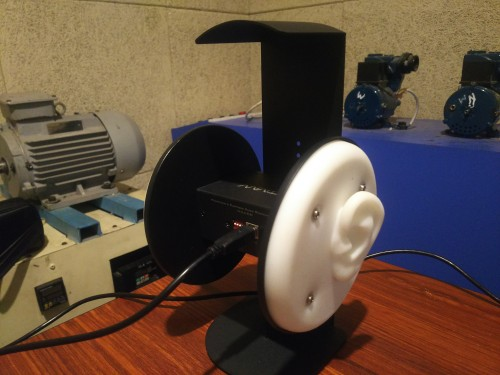
\includegraphics[width=200pt]{images/ears}
			\caption{miniDSP EARS}
		\end{figure}
	
		Untuk selanjutnya, paket intrumen ini disebut EARS saja.
		
		\item Focusrite dan Microphone (menyusul)
		
		Untuk selanjutnya paket instrumen ini disebut Mic saja
		
		\item Pistonphone Calibrator IEC942 dengan frekuensi 1000Hz dan loudness 114dB SPL sebagai acuan kalibrasi.
		\begin{figure}[!ht]
			\centering
			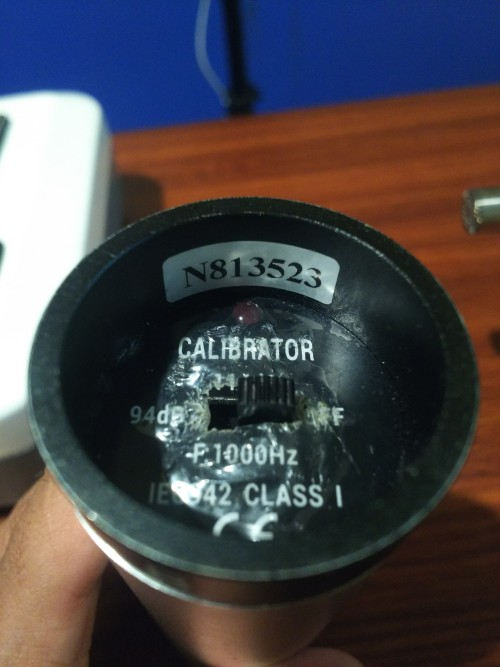
\includegraphics[width=200pt]{images/calibrator}
			\caption{Calibrator}
		\end{figure}	
\end{itemize} 
	
	\subsection{Kalibrasi}
	
	Proses kalibrasi dilakukan untuk dua paket intrumen, yaitu EARS dan Mic.
	
	\subsubsection{EARS}
	
	Langkah kalibrasi EARS meliputi:
	\begin{enumerate}
		\item Lepas semua telinga karet sehingga internal microphone bisa ter-\textit{expose}
		\item Pastikan semua switch diatur untuk gain 0dB.
		\item Sambungkan USB ke laptop.
		\begin{enumerate}
			\item Untuk sistem operasi GNU/Linux, pastikan input Pulseaudio adalah EARS (bukan internal mic)
			\item Nyalakan software DSSF3, pilih FFT Analyzer
			\item Untuk sistem operasi Windows, pilihan input akan tampil disini (pilih EARS).	
	\end{enumerate}
		\item Klik \textbf{Calibration} untuk menampilkan jendela kalibrasi.
		Pilih \textbf{Separate} untuk kalirasi sisi kanan dan kiri.
		\begin{figure}[!ht]
			\centering
			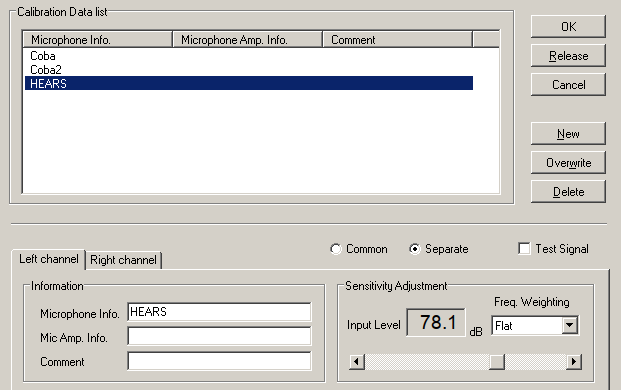
\includegraphics[width=200pt]{images/kalib}
			\caption{Jendela Kalibrasi}
		\end{figure}
		\item Masukkan microphone ke kalibrator.
		\begin{figure}[!ht]
			\centering
			\begin{subfigure}[b]{0.25\textwidth}
				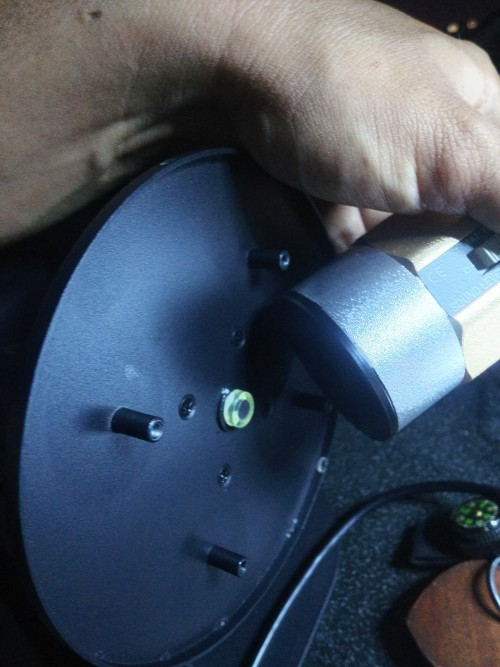
\includegraphics[width=\textwidth]{images/ears_calib0}
			\end{subfigure}
			\begin{subfigure}[b]{0.25\textwidth}
				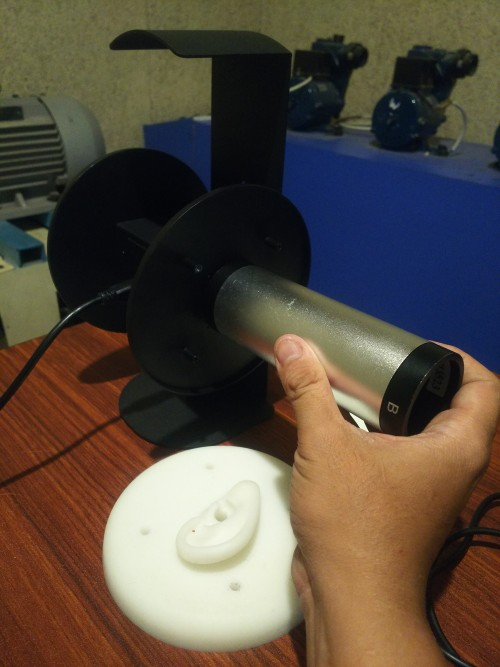
\includegraphics[width=\textwidth]{images/ears_calib1}
			\end{subfigure}
			\caption{Kalibrasi EARS}
		\end{figure}
		\item Geser slider kalibrasi hingga menunjukkan angka 114dB
		\item Ulangi untuk microphone di sisi lainnya.
		\item Beri nama pada \textbf{Microphone Info} dan klik \textbf{New} untuk menyimpan.
	\end{enumerate}

	\subsubsection{Mic}
	
	Menyusul
	
	\subsection{Pengukuran latar}
	
\end{document}